\documentclass[11pt,fleqn,twoside]{article}
\usepackage{makeidx}
\makeindex
\usepackage{palatino} %or {times} etc
\usepackage{plain} %bibliography style 
\usepackage{amsmath} %math fonts - just in case
\usepackage{amsfonts} %math fonts
\usepackage{amssymb} %math fonts
\usepackage{lastpage} %for footer page numbers
\usepackage{fancyhdr} %header and footer package
\usepackage{mmpv2} 
\usepackage{url}
\usepackage{float}

% the following packages are used for citations - You only need to include one. 
%
% Use the cite package if you are using the numeric style (e.g. IEEEannot). 
% Use the natbib package if you are using the author-date style (e.g. authordate2annot). 
% Only use one of these and comment out the other one. 
\usepackage{cite}
\usepackage[parfill]{parskip}
%\usepackage{natbib}

\begin{document}

\name{Aidan Wynne Fewster}
\userid{awf1}
\projecttitle{NHS Wales Injectable Medicine Guide Android application}
\projecttitlememoir{NHS Wales Android application} %same as the project title or abridged version for page header
\reporttitle{Design Specification}
\version{1.0}
\docstatus{Release}
\modulecode{CS39440}
\degreeschemecode{G400}
\degreeschemename{Computer Science}
\supervisor{Andrew Starr} % e.g. Neil Taylor
\supervisorid{aos}
\wordcount{}

%optional - comment out next line to use current date for the document
%\documentdate{10th February 2014} 
\mmp

\setcounter{tocdepth}{3} %set required number of level in table of contents


%==============================================================================
\section{Introduction}
%==============================================================================
\subsection{Purpose of this document}
%==============================================================================\
The purpose of the document is to provide documentation for the architectural design of the NHS Wales injectable medicines guide Android application.  It will show the class's which should be created and the methods within them, as well as how they're linked, this will be achieved through a class diagram. This document will also outline the project user interface design through UI mock-up wireframes.


%==============================================================================
\subsection{Project overview}
%==============================================================================
The main focus of this project is to produce a application for Android which will aid NHS medical staff in obtaining information on injectable medicines. The user will be able to search through a list of drugs by there title. Upon selecting a drug they will be able to view a detailed monograph for that drug. User will also be able to calculate dosage and infusion rates using the application.

%==============================================================================
\section{Architectural design}
%==============================================================================
The application will be split up into separate packages, each performing a specific task. These packages will be called named activities, data download, database and the models package.

Separating the classes in related modules improves the re-usability and maintainability of the code. As future developers will easily be able to find the task of each class from its module.

The following sections will state the overall use case and provide class diagrams for each module.
\newpage
%==============================================================================
\subsection{Use case diagram}
%==============================================================================

\begin{figure}[H]
\centering
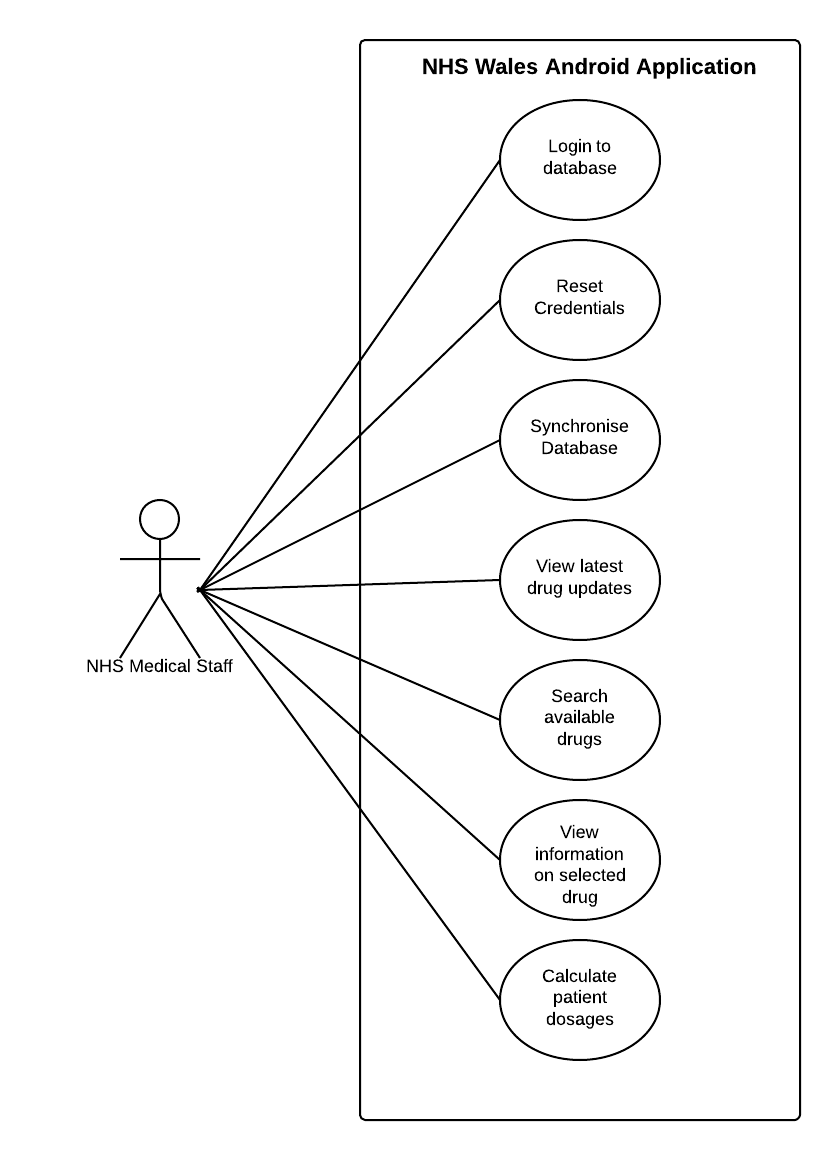
\includegraphics[width=4.5in]{useCase}
\caption{Use case diagram for the application}
\end{figure}

%==============================================================================
\subsubsection{Use case descriptions}
%==============================================================================
\begin{description}
	\item[Login to database]  A user will be able to authenticate themselves with the database using their NHS login credentials.
	\item[Synchronise database] Upon authenticating themselves the user will be able to download a complete copy of the available database to their device.
	\item[View latest drug updates] The user will how many monographs have been added or removed from the live database since they last synchronised their local one.
	\item[Search available drugs] The user will be able to easily search through all the drugs within the database. The search will automatically suggest suitable results.
	\item[View information on selected drug] Upon selecting a drug the user will be able to view a monograph for that drug. They will be able to select each section of the monograph they would like to read.
	\item[Calculate patient dosages] The user will be able to calculate the infusion rate and dosage for a given patient. This information will be validated for user input error. 
\end{description}

%==============================================================================
\subsection{Models package class diagram}
%==============================================================================
The models package contains the model classes for each of the database tables. A model represents an item created from the database, for example a drug or a piece of information about a drug. Keeping all models within one package allows the models to be reused in other applications.

\begin{figure}[H]
\centering
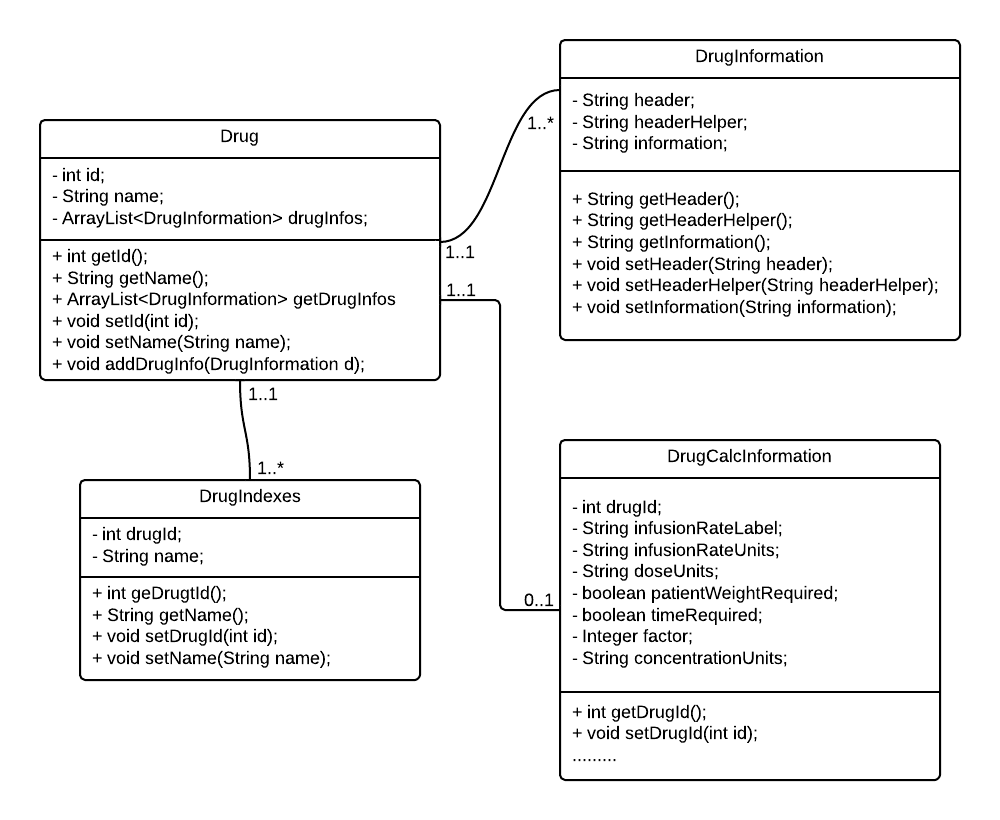
\includegraphics[width=6.5in]{models}
\caption{Class diagram for the models package}
\end{figure}

%==============================================================================
\subsubsection{Class diagram descriptions}
%==============================================================================
\begin{description}
	\item[Drug] This class represents a drug in the database
	\item[DrugIndex] This class represents a drug index, a drug index is a searchable name for a drug.
	\item[DrugInformation] This class represents a piece of the monographs information about the drug.
	\item[DrugCalcInformation] This class a set of information needed to perform a calculation
\end{description}

%==============================================================================
\subsection{Database package class diagram}
%==============================================================================
This package contains all classes that interact with the SQLite database. Currently this package only contains one class, but if the application expands, more classes can be added to split up the classes.

\begin{figure}[H]
\centering
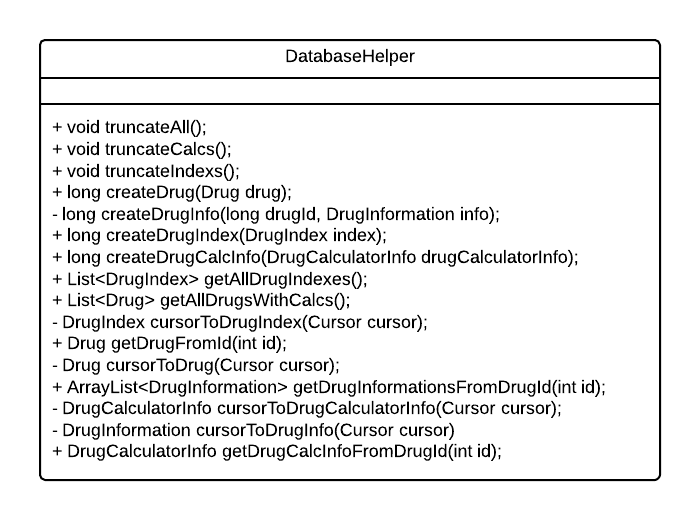
\includegraphics[width=6.5in]{database}
\caption{Class diagram for the database package}
\end{figure}

%==============================================================================
\subsubsection{Class diagram descriptions}
%==============================================================================
\begin{description}
	\item[DatabaseHelper] This class is responsible for fetching, creating and deleting data from the database. Having this class within its own package will allow the database and database code to be reused within other applications. If the code within the database helper class becomes to large using a package will also allow the code to be broken into smaller classes.
\end{description}

%==============================================================================
\subsection{Activities package class diagram}
%==============================================================================
Activities are Android's views. An activity provides a method of displaying information on screen for the user. The activities package contains the implemented classes for the activities. 

\begin{figure}[H]
\centering
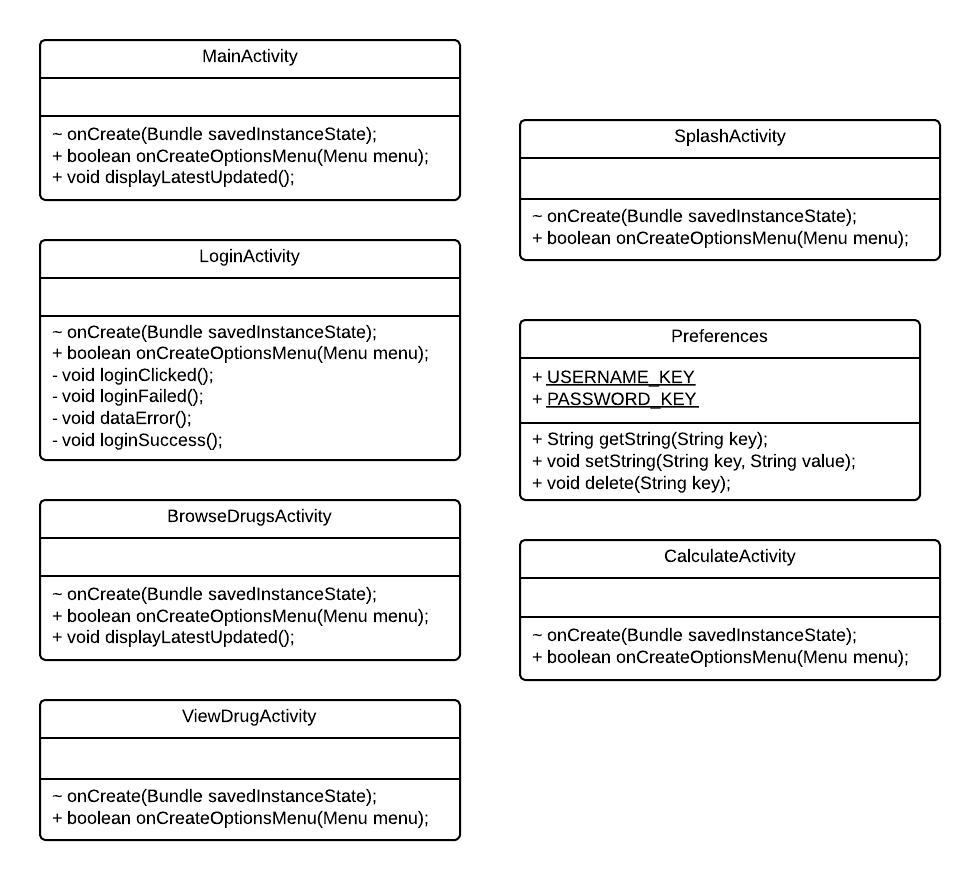
\includegraphics[width=6.5in]{activities}
\caption{Class diagram for the activities package}
\end{figure}

%==============================================================================
\subsubsection{Class diagram descriptions}
%==============================================================================
\begin{description}
	\item[MainActivity] Shown once the user has successfully downloaded the database. This is the first screen a reoccurring user is sent to. This page allows the user to navigate to other screens.
\	\item[LoginActivity] This is the first screen the user sees when opening the application for the first time. Once they login their details are saved so they should only have to login once.
	\item[DownloadActivity]
	This page is shown when the user is downloading the database for the first time, or when they are updating the database. The tasks within this screen can take several minutes so a progress bar helps to show to the user that the task is still running and hasn’t crashed.
	\item[BrowseDrugsActivity]
	These two screens are very similar; they both display a list of drugs and allow you to filter the list by entering part of the drugs name, inside the search box. The browse drugs page contains a list of all drugs and the browser calculators screen shows all drugs that have calculators.
	\item[ViewDrugActivity]
	This screen is displayed when the user selects a drug from the browse drugs page. It contains the complete monograph for the drug, some headers contain an icon next to the header, if the user clicks a head with this icon, and helper information for that header is displayed within a dialog.
	\item[Calculator screen]
	This is the screen where the user enters patient information and is displayed with the either the dose or infusion rate for the drug. When the result of the calculation is displayed, the equation used to perform the calculation is also displayed and described.
\end{description}


%==============================================================================
\subsection{Data download package class diagram}
%==============================================================================
The data download package contains the Robospice requests classes, which are responsible for downloading the individual API URLs and then parsing the data obtained. Each class within this package downloads a specific API XML file. Having all the data download classes in one package makes it easy to add new classes to download additional data in the future.

\begin{figure}[H]
\centering
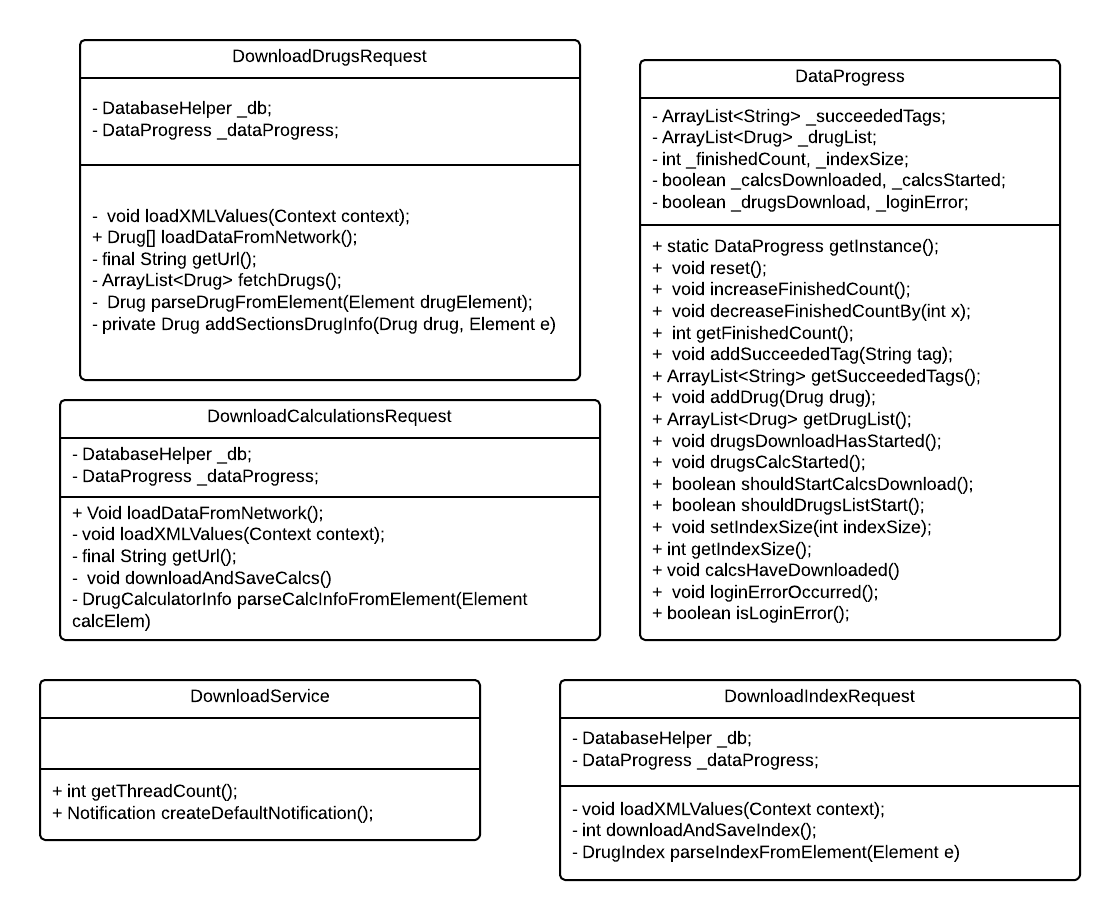
\includegraphics[width=6.5in]{download}
\caption{Class diagram for the data download package}
\end{figure}

%==============================================================================
\subsubsection{Class diagram descriptions}
%==============================================================================
\begin{description}
	\item[DataProgress] This is class is used for checking the progress of requests and for displaying errors within the data download activity. This is a singleton class, so only one object of this class can be nstantiated.
\	\item[DownloadCalculationsRequest] This class is responsible for downloading the drug calculator informations
	\item[DownloadDrugsRequest] This class is responsible for downloads the drugs and their informations
	\item[DownloadDrugIndex] This class is responsible for downloading the drug indexes
	\item[DownloadService] RobospiceService class for handling the download of data. This is an uncached service as the data is downloaded infrequently, so the cache will most likely have expired by the next time the request is made.
\end{description}

\end{document}
